%%%%%%%%%%%%%%%%%%%%%%%
%%%%%%%% EPL %%%%%%%%%%
%%%%%%%%%%%%%%%%%%%%%%%

\documentclass[doublecol,final]{epl2}

\usepackage{amsmath}

\usepackage{amssymb}

\makeatletter
\setlength\arraycolsep{2pt}
\makeatother

\vol{110}
\issue{1}
\year{2015}
\firstpage{1}
\doi{10.1209/0295-5075/110/27001}
\pgid{27001}
\received{30 January 2015}
\acceptedinfinalform{7 April 2015}
\paperpub{April 2015}
\onlinepub{30 April 2015}

\title{Long-lived spin coherence of indirect excitons in GaAs coupled\\ quantum wells\vspace*{-7pt}}

\shorttitle{Long-lived spin coherence of indirect excitons in GaAs coupled quantum wells}

\author{Mussie Beian\inst{1}, Mathieu Alloing\inst{1,3}, Edmond Cambril\inst{2}, Carmen Gomez Carbonell\inst{2}, Johann Osmond\inst{1}, Aristide Lema\^{i}tre\inst{2} \and Fran\c{c}ois Dubin\inst{1,3}\thanks{E-mail: \email{francois.dubin@insp.jussieu.fr}}}

\shortauthor{Mussie Beian \etal}

\institute{
\inst{1} ICFO-The Institute of Photonic Sciences - Av. Carl Friedrich Gauss, num. 3, 08860 Castelldefels, Spain\\
\inst{2} Laboratoire de Photonique et Nanostructures, LPN/CNRS - Route de
Nozay, 91460 Marcoussis, France\\
\inst{3} Institut des Nanosciences de Paris, CNRS and UPMC - 4 pl. Jussieu,
75005 Paris, France}

\abstract{~We study spatially indirect excitons confined in a symmetric GaAs double quantum well. We show that the spin polarisation of very dilute gases can be optically imprinted, in both pure and superposition states. In the regime where indirect excitons can be localized, we observe at 350\un{mK} that the excitons spin degree of freedom is frozen with a relaxation time comparable to the coherence time and to the radiative lifetime $(\sim 30\un{ns})$.}

\pacs{73.63.Hs}{Quantum wells}
\pacs{78.47.jd}{Time resolved luminescence}

\begin{document}

\maketitle

Over the last decade, the spin degree of freedom of semiconductor excitons has been intensively studied, both \nobreak{experimentally} and theoretically. The mechanisms responsible for excitons spin flips have first been identified in the regime where excitons are delocalised. These include momentum scatterings to flip electron spins, energy relaxation in the valence bands to flip hole spins as well as inter-band Coulomb (exchange) scatterings~\cite{epl17031bib1,epl17031bib2,epl17031bib3,epl17031bib4}.~Usually, they lead to short $(\sim 100\un{ps})$ exciton spin relaxation times~\cite{epl17031bib5,epl17031bib6,epl17031bib7}. By contrast, in the regime where excitons are confined in every direction, \textit{e.g.} in a quantum dot, the spin relaxation is damped by the quantisation of the excitons momentum and its resulting distribution of accessible energy states. Excitonic spins can then be ``frozen'' with a relaxation time increased to about 10\un{ns}~\cite{epl17031bib8}, \textit{i.e.} an order of magnitude longer than the excitons radiative lifetime $(\sim1\un{ns})$, which actually sets an upper bound for spin manipulations. Localized excitons with a long radiative lifetime are in fact among the most promising candidates to develop semiconductor architectures for quantum information \nobreak{science}~\cite{epl17031bib9}.

The lifetime of semiconductor excitons may be directly tuned through the spatial overlap between the excitons constituents. This is notably achieved in electrically biased coupled quantum wells where one enforces a spatial separation between electrons and holes. Thus, spatially indirect excitons are engineered. Here, we show that \nobreak{indirect} excitons have a long-lived spin coherence, of the order of the radiative lifetime $(\sim 30\un{ns})$. This is achieved below a few kelvins in a very dilute regime where indirect excitons can be localized. Thus, we observe that photo-injected electrons and holes have a frozen spin. This allows us to program all-optically arbitrary spin polarizations for indirect excitons, \textit{e.g.} pure or superposition states. Let us then note that our experiments are performed on a spin ensemble distributed over $\approx 5\un{\mu m}$. The average spin polarisation is then manipulated at an efficiency \textit{a priori} limited by inhomogeneous broadening, \textit{i.e.} by the spatial variations of the effective magnetic field acting on individual spins. We therefore expect our degree of control to be significantly enhanced at the single-exciton level using the appropriate technology~\cite{epl17031bib10}.

\looseness-1To probe the excitons spin degree of freedom, polarisation-resolved photoluminescence provides a direct and handful approach~\cite{epl17031bib1,epl17031bib2,epl17031bib3}:~Photoluminescence results from the recombination of optically active states $(|\pm1\rangle)$, \textit{i.e.} with a total ``spin'' $(\pm 1)$. A spin flip of either of the exciton constituents, $(\mp 1/2)$ electron or $(\pm 3/2)$ hole, converts these bright excitons into optically inactive (dark) ones, \textit{i.e.}~with a total spin $(\pm 2)$. This yields a loss of photoluminescence.~By contrast electron-hole exchange, \textit{i.e.}~a simultaneous spin flip of both electron and hole, turns a~bright exciton with a spin $(+1)$ into a bright exciton with, however, a spin $(-1)$, or vice versa.~Individual carrier spin flips as well as electron-hole exchange then \nobreak{control} the \nobreak{dynamics} of polarisation-resolved \nobreak{photoluminescence}~\cite{epl17031bib1}, \textit{i.e.}~of the, $|+1\rangle$ and $|-1\rangle$, populations of bright\break excitons.

The dynamics of exciton spins have been well highlighted in GaAs quantum wells through time-resolved photoluminescence. It has revealed electronic spin flips through a multi-component decay in polarisation-resolved spectroscopy (characteristic timescales are in the range of tens to hundreds of picoseconds~\cite{epl17031bib1,epl17031bib2,epl17031bib3,epl17031bib5}). In coupled quantum wells (CQWs) where electrons and holes are spatially separated, the spin relaxation of indirect excitons has been found very different~\cite{epl17031bib11,epl17031bib12,epl17031bib13}. Experiments have shown that when prepared in a pure state $(|\pm1\rangle)$, indirect excitons exhibit a very long-lived polarisation~\cite{epl17031bib14} with a time decay that can even exceed the radiative lifetime $(\approx 100\un{ns})$, \textit{i.e.} orders of magnitude more than direct excitons or free electrons~\cite{epl17031bib15}. In this letter, we extend this degree of control. We show that the spin of indirect excitons can be prepared in coherent superpositions, \textit{i.e.} with a linear polarisation such as $|H\rangle\equiv (|1\rangle+|-1\rangle)$ or $|V\rangle\equiv (|1\rangle-|-1\rangle)$. Thus, we evidence a regime where the spin degree of freedom of photo-injected electronic carriers is frozen and the excitons spin coherence protected.

\begin{figure}%fig1
\centering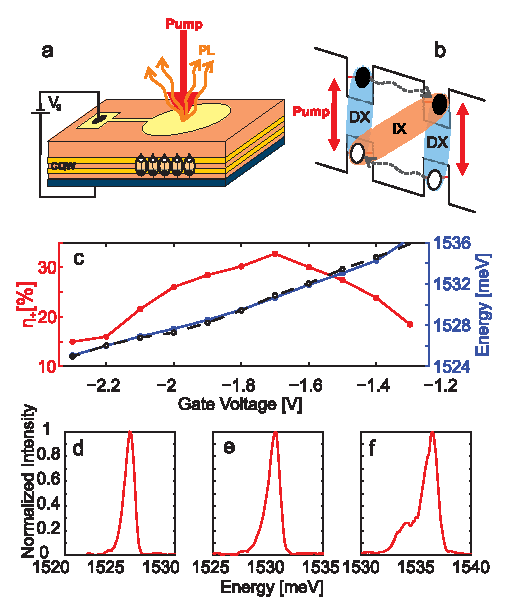
\includegraphics{epl17031f1_pr.eps}
\caption{(Colour on-line) (a),~(b): schematic representation of our experiments. Direct excitons (DX) are quasi-resonantly excited by a pump pulse which leads to indirect excitons (IX) once electronic carriers have tunnelled towards minimum \nobreak{energy} states. Photoluminescence (PL) emitted by indirect excitons is then analysed. (c) Degree of spin polarisation $(\eta_{+})$ \textit{vs.} the applied gate voltage $V_{g}$ together with the energy of the $\sigma^{+}$ and $\sigma^{-}$ polarised photoluminescence, black and blue, respectively. (d)--(f): photoluminescence spectra emitted for $V_g= \{-2.3,-1.7,-1.4\}\ \mathrm{V}$ (from left to right). Measurements have been realised at 350\un{mK} and acquired in the illuminated region, in a 10\un{ns} time interval starting 10\un{ns} after extinction of the laser excitation.}\label{epl17031fig1}
\end{figure}

Figure~\ref{epl17031fig1}(a),~(b) provides a sketch of our experiments: We study indirect excitons confined in a $50\un{\mu m}$ wide disk-shaped electrostatic trap of a symmetric GaAs CQW (the CQW consists of two 8\un{nm} wide GaAs quantum wells separated by a 4\un{nm} $\mathrm{Al}_{.33}\ \mathrm{Ga}_{.67}$As barrier).~It is placed 100\un{nm} above a n-doped GaAs substrate serving as ground electrode whereas the strength of the electric field in the plane of the CQW is controlled by the static bias $(V_g)$ applied on the surface semi-transparent electrode located 900\un{nm} above the CQW. In our experiments, electronic carriers are directly injected in the trap using 50\un{ns} long laser pulses (at 4\un{MHz} repetition rate).~This pump laser is slightly red-detuned from the resonance of the direct excitonic transition of each quantum well. It is focussed down to $\sim 4\un{\mu m}$ and in most of the following experiments the mean optical power is set to 100\un{nW} such that we restrict our studies to very dilute gases. Varying the polarisation of the pump laser we control the spin polarisation of direct excitons injected in the two quantum wells. Energy relaxation then leads to the formation of indirect excitons (fig.~\ref{epl17031fig1}(b)) with a spin polarisation that can reflect the initial laser polarisation.

Figure~\ref{epl17031fig1}(c) shows the efficiency at which $(+1)$ spin-polarised indirect excitons are created after a $\sigma^+$ \nobreak{polarized} pump pulse, as a function of $V_{g}$. The degree of polarisation, $\eta_{+}= (I_{\sigma^+}-I_{\sigma^-})/(I_{\sigma^+}+I_{\sigma^-})$ with $I_{(\sigma^+,\sigma^-)}$ being the integrated intensity of the $(\sigma^+,\sigma^-)$ polarised photoluminescence, is measured only in the illuminated region and 10\un{ns} after extinction of the pump laser, as for most of our experiments. Overall $\eta_{+}\geq 15{\%}$ reveals that the spin polarization is significant and long-lived. In addition, we note that $\eta_{+}$ exhibits a non-monotonic dependence with $|V_g|$: it first increases to reach its $\approx 32{\%}$ maximum at $V_g = -1.7\un{V}$, before it decreases for larger gate voltages. This behaviour may first be related to the dependence of the electron and hole inter-well tunnelling with the applied gate voltage: Varying $V_g$ one modifies the tunnelling rate of electrons and holes between the two quantum wells of our heterostructure~\cite{epl17031bib16}. The spin polarisation of indirect excitons being only established when the carriers tunnelling time is fast compared to their spin relaxation time, one cannot exclude that the variation of $\eta_+$ with $V_g$ results from modified electrons and holes tunnelling rates between the two quantum wells. At the same time, the electron~(hole) spin relaxation also depends on $V_g$~\cite{epl17031bib1} which hinders the mechanisms ruling the excitons spin \nobreak{polarisation}.

\looseness-1To further study the excitons spin polarisation, we analysed the photoluminescence spectra for particular gate voltages, $V_g= \{-1.4,-1.7,-2.3\}\un{volts}$.~As shown in fig.~\ref{epl17031fig1}(d)--(f), these display two components: A high-energy emission due to the recombination of indirect excitons, and a second contribution at lower energy reflecting the interaction between indirect excitons and excess carriers~\cite{epl17031bib17}. The latter emission is usually referred to as charged exciton line and for our field-effect device excess carriers are most probably electrons from the leakage current $(\sim\text{nA})$. Interestingly, fig.~\ref{epl17031fig1}(d)--(f) signals that the relative weight between the two components of the spectrum varies strongly in the range of $V_{g}$ that we explored. Precisely, increasing $|V_g|$ the amplitude of the low-energy emission is continuously reduced. This manifests the decrease of the concentration of excess electrons interacting with indirect excitons, \textit{i.e.} that electro-neutrality is better fulfilled in the CQW. The spin polarisation being best imprinted for $V_{g}= -1.7\un{V}$, \textit{i.e.} somewhat in the middle of this range, we may conclude, as for two-dimensional electron gases~\cite{epl17031bib18}, that at this particular setting excess electrons contribute to the damping of spin relaxation channels. This may be achieved through localisation of indirect excitons. In such a case, electric-field--induced modifications of spin-orbit interactions~\cite{epl17031bib4,epl17031bib19} would not be dominant. This conclusion is further supported by the weak variation (within our instrumental precision of $\sim 100\un{\mu eV}$) of the energy splitting between $|+1\rangle$ and $|-1\rangle$ energy levels\break (fig.~\ref{epl17031fig1}(c)).

\begin{figure}%fig2
\centering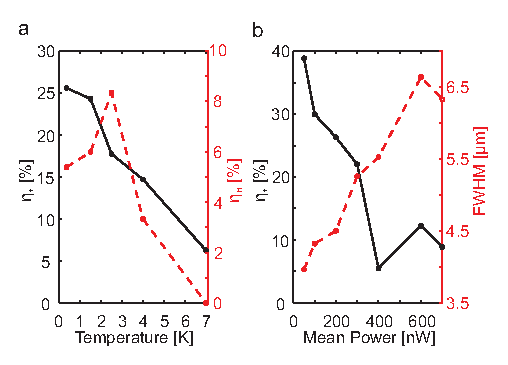
\includegraphics{epl17031f2_pr.eps}
\caption{(Colour on-line) (a) Variation of the degree of \nobreak{circular} polarisation ($\eta_{+}$, solid black line) and linear polarisation ($\eta_{H}$, dashed red line) as a function of the bath temperature. (b)~Variation of $\eta_{+}$ as a function of the excitation mean power (solid black line) together with the spatial full width at half-maximum (FWHM) of the exciton gas (dashed red line). Measurements were performed at $V_g= -1.7\un{V}$ and at 350\un{mK}. They were recorded in the illuminated region, 10\un{ns} after \nobreak{extinction} of the pump laser. In (a) the mean optical was set to 100\un{nW}.}
\label{epl17031fig2}
\end{figure}

In a subsequent experiment, we measured $\eta_{+}$ while increasing the bath temperature which we used to promote exciton delocalisation. The results are displayed in fig.~\ref{epl17031fig2}(a) and show that the degree of spin polarisation drops rapidly above $\sim 2\un{K}$, \textit{i.e.} when the thermal activation energy is about $150\un{\mu eV}$. This value well compares to the amplitude of structural disorder that we can estimate from the line width of the direct exciton emission $(\sim 400\un{\mu eV})$. We then performed a control \nobreak{experiment} by keeping our device at the lowest bath temperature (350\un{mK}) while the exciton density is increased with the power of our laser excitation. Hence, we increase the strength of repulsive dipolar interactions between excitons yielding a screening of intrinsic disorder (structural or \nobreak{electrostatic}) and a triggering of the spatial extension (\nobreak{delocalisation}) of the exciton gas~\cite{epl17031bib20,epl17031bib21,epl17031bib22}. As for an increase of the bath temperature, fig.~\ref{epl17031fig2}(b) signals that enhancing the exciton density also leads to a rapid decrease of the degree of spin polarisation. Precisely, the spin polarisation almost vanishes, at the position of the laser excitation, when the strength of the drift-diffusion induced by dipolar interactions suffices to initiate the expansion of the cold gas. Our observations are then in striking contrast with recent experiments reporting the transport of spin-polarised indirect excitons~\cite{epl17031bib23}. In agreement with recent works\cite{epl17031bib13}, here the spin polarisation is best established when excitons are efficiently isolated, \textit{i.e.} at the lowest density and bath temperature. In this regime we estimate that the density does not exceed $\sim 10^9\un{cm^{-2}}$ since we do not resolve any blue-shift of the photoluminescence while the density is increased. Weak intrinsic disorder $(\sim 100\un{\mu eV})$ then prevents excitons from following a continuous bi-dimensional density of states~\cite{epl17031bib20,epl17031bib21} and excitons are effectively \nobreak{localised}.

Above, we have shown that indirect excitons can be prepared in a pure spin state, \textit{i.e.} $|\pm1\rangle$. Creating superposition states is more demanding since these require a well-defined phase relation between the two $|\pm1\rangle$ spin components, \textit{e.g.} horizontal and vertical polarisations $|H\rangle\equiv (|1\rangle+ |-1\rangle)$ and $|V\rangle\equiv(|1\rangle-|-1\rangle)$, respectively. Their successful programmation first implies that a linearly polarised pump pulse allows us to set a linear spin polarisation for direct excitons. While this \nobreak{prerequisite} shall be fulfilled~\cite{epl17031bib7}, electronic carriers will have to \nobreak{maintain} the phase of their spin degree of freedom while tunnelling between the two quantum wells. Thus, indirect excitons can be prepared in a superposition spin state. In fig.~\ref{epl17031fig3} we show that this control is achievable: By setting the appropriate linear polarisation for the pump laser, we create horizontally or vertically spin-polarised indirect excitons. Let us note that the programmed linear polarisation does not depend on the crystallographic axis, we actually verified that linear spin polarisations can be imprinted along arbitrary directions solely by tuning the polarisation of the pump laser.~Furthermore, the spin polarisation is long-lived since the data in fig.~\ref{epl17031fig3} was recorded 10\un{ns} after extinction of the excitation. In these experiments, we reached a fidelity, $\eta_H\sim\eta_V= 6{\%}$, that directly follows from the efficiency at which we created pure states since $\eta_H=\eta_\mathrm{\sigma^+}\eta_{\sigma^-}\ (\eta_+\sim \eta_- \sim 0.25$ for these measurements, see fig.~\ref{epl17031fig3}(a),~(b)). In fact, we observed that the efficiency of our optical programation is bound to $\sim 10{\%}$ for superposition states (\textit{e.g.} in fig.~\ref{epl17031fig2}). The experiments displayed in fig.~\ref{epl17031fig3}(c),~(d) nevertheless underline a coherent electron (hole) inter-well tunnelling where spin coherence is preserved, otherwise we could not create horizontal or vertical spin polarisations. Interestingly, we note that \nobreak{coherent} inter-well tunnelling has recently been reported for electrically polarised exciton-polaritons~\cite{epl17031bib24}.

We assessed the relaxation and coherence times of exciton spins in a last experiment where we monitored the \nobreak{dynamics} of the photoluminescence emitted by a $(\pm 1)$ spin-polarised gas, or by a gas with linear ($H$ or $V$) spin polarisation, in order to infer both the spin relaxation and diffusion, respectively. We performed these measurements in the very dilute regime where we program excitonic spins with highest fidelities. Figure~\ref{epl17031fig4} displays our experimental results. We quantify these using the theoretical framework introduced by Sham and co-workers~\cite{epl17031bib1}. It is based on a set of rate equations ruling the dynamics of populations in each of the four magnetic levels (the two $|\pm1\rangle$ bright excitons and the dark ones $|\pm2\rangle$). These are linearly coupled by individual carrier spin flips as well as electron-hole exchange, at rates ruling the dynamics of the photoluminescence polarisation.

\begin{figure}%fig3
\centering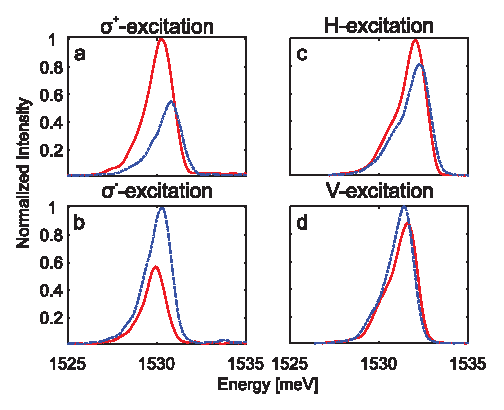
\includegraphics{epl17031f3_pr.eps}
\caption{(Colour on-line) Photoluminescence spectra with circular right and circular left polarisations (solid red and dashed blue lines, respectively) for a $\sigma^+$ polarised laser excitation~(a) and for a $\sigma^-$ polarised excitation (b). Photoluminescence spectra with horizontal and vertical polarisations (solid red and dashed blue lines, respectively) for horizontally (c)~or vertically polarised (d) excitations.~The measurements have been realised at $V_g =-1.7\un{V}$ at 350\un{mK} and acquired in the \nobreak{illuminated} region 10\un{ns} after termination of the laser \nobreak{excitation.}}
\label{epl17031fig3}
\end{figure}

\begin{figure}%fig4
\centering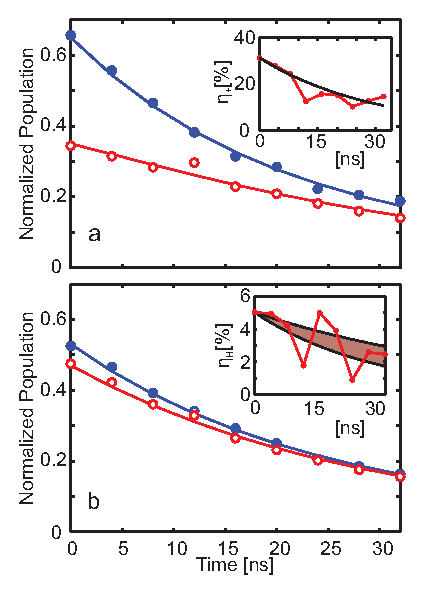
\includegraphics{epl17031f4_pr.eps}
\caption{(Colour on-line) (a) Dynamics of populations with $(+1)$ and $(-1)$ spins (blue and red, respectively). The inset displays the decay of the spin polarisation, fitted by a single exponential with a 30\un{ns} $(T_1)$ decay time. (b) Dynamics of the transverse spin populations with $H$ and $V$ polarisations (blue and red, \nobreak{respectively}). The degree of linear spin polarisation is displayed in the inset together with mono-exponential decays with decay times $T_1$ and $2T_1$. In (a) and (b) lines correspond to the best fit for the experimental data. Measurements were realised at 350\un{mK} for $V_g= -1.7\un{V}$, restricted to the illuminated region, with a 2\un{ns} time resolution while laser pulses were terminated at time 0.}
\label{epl17031fig4}
\vspace*{-10pt}
\end{figure}

\looseness-1As shown in fig.~\ref{epl17031fig4}, the excitons dynamics is best fitted with two dominant time decays, namely $T_1$ and $T_2$ for the relaxation of pure and transverse (coherent) spin polarisations, respectively. For our experiments, we deduce $T_1 \sim T_2 \sim 30\un{ns} \ \sim\tau_R$, $\tau_R$ being the radiative lifetime.~Within the precision of our fitting routine, we cannot distinguish these parameters with good confidence. Figure~\ref{epl17031fig4}(a) then confirms that indirect excitons have a long-lived longitudinal spin relaxation~\cite{epl17031bib14,epl17031bib15}, but more interestingly fig.~\ref{epl17031fig4}(b) shows that they also exhibit a long-lived spin coherence. The latter property implies that individual carrier spin flips are frozen otherwise coherence would be lost~\cite{epl17031bib4}. In fact, we estimate that electron or hole spin flips only occur on a slow timescale $(\gg 100\un{ns})$ which cannot be extracted more precisely from our numerical analysis. To the best of our knowledge, such \nobreak{extended} relaxation times had not been expected \nobreak{theoretically}~\cite{epl17031bib25}. Finally, let us stress that the weak degree of linear \nobreak{polarisation} does not allow us to extract accurately the excitons spin coherence time (see inset in fig.~\ref{epl17031fig4}(b)). We observe that $T_1\leq T_2\leq 2T_1$ such that we can hardly discuss quantitatively the role of pure dephasing.

To conclude we have shown, in the regime where localisation is important and at sub-kelvin temperatures, that indirect excitons have a spin degree of freedom which is frozen. It can then serve for coherent memory applications, the storage decay time reaching $\sim 30\un{ns}$ in our \nobreak{experiments} limited by inhomogeneous broadening.~At the single-exciton level, \textit{e.g.} in a sub-micron wide electrostatic trap~\cite{epl17031bib10}, spin coherence shall then be increased. Combined to more efficient initialisations, this approach could pave the way towards interesting applications in quantum information science.

\acknowledgments{\vspace*{-7pt}This work has been supported by the EU-ITN INDEX and EU-CIG X-BEC. The authors thank \textsc{B. Eble} for a critical reading of the manuscript.}

\begin{thebibliography}{99}

\bibitem{epl17031bib1}
\Name{Mazaille M. Z., de Andreada e Silva E. A. \and Sham~L. J.}
\REVIEW{Phys. Rev. B}{47}{1993}{15776}.

\bibitem{epl17031bib2}
\Name{Vinattieri A. \etal}
\REVIEW{Phys. Rev. B}{50}{1994}{10868}.

\bibitem{epl17031bib3}
\Name{Vina L.}
\REVIEW{J. Phys.: Condens. Matter}{11}{1999}{5929}.

\bibitem{epl17031bib4}
\Name{Wu M. W., Jiang J. H. \and Weng M. Q.}
\REVIEW{Phys. Rep.}{493}{2010}{236}.

\bibitem{epl17031bib5}
\Name{Bar-Ad S. \and Bar-Joseph I.}
\REVIEW{Phys. Rev. Lett.}{68}{1992}{349}.

\bibitem{epl17031bib6}
\Name{Damen T. C., Vina L., Cunningham J. E., Shah J. \and Sham L. J.}
\REVIEW{Phys. Rev. Lett.}{67}{1991}{3432}.

\bibitem{epl17031bib7}
\Name{Marie X. \etal}
\REVIEW{Phys. Rev. Lett.}{79}{1997}{3222}.

\bibitem{epl17031bib8}
\Name{Paillard M. \etal}
\REVIEW{Phys. Rev. Lett.}{86}{2001}{1634}.\vadjust{\vspace*{36.6pc}\pagebreak}

\bibitem{epl17031bib9}
\Name{Poem E. \etal}
\REVIEW{Nat. Phys.}{6}{2010}{993}.

\bibitem{epl17031bib10}
\Name{Schinner G. \etal}
\REVIEW{Phys. Rev. Lett.}{110}{2013}{127403}.

\bibitem{epl17031bib11}
\Name{Aichmayr G. \etal}
\REVIEW{Phys. Rev. Lett.}{83}{1999}{2433}.

\bibitem{epl17031bib12}
\Name{Larionov A. V.}
\REVIEW{Phys. Rev. B}{73}{2006}{235329}.

\bibitem{epl17031bib13}
\Name{Leonard J. R. \etal}
\REVIEW{Nano Lett.}{9}{2009}{4204}.

\bibitem{epl17031bib14}
\Name{Kowalik-Seidl K. \etal}
\REVIEW{Appl. Phys. Lett.}{97}{2010}{011104}.

\bibitem{epl17031bib15}
\Name{Andreakou P. \etal}
\REVIEW{Phys. Rev. B}{91}{2015}{125437}.

\bibitem{epl17031bib16}
\Name{Poggio M. \etal}
\REVIEW{Phys. Rev. B}{70}{2004}{121305(R)}.

\bibitem{epl17031bib17}
\Name{Alloing M. \etal}
\REVIEW{EPL}{107}{2014}{10012}.

\bibitem{epl17031bib18}
\Name{Chen Z. \etal}
\REVIEW{Nat. Phys.}{3}{2007}{265}.

\bibitem{epl17031bib19}
\Name{Balocchi A. \etal}
\REVIEW{Phys. Rev. Lett.}{107}{2011}{136604}.

\bibitem{epl17031bib20}
\Name{Alloing M., Lema\^{i}tre A. \and Dubin F.}
\REVIEW{EPL}{93}{2011}{17007}.

\bibitem{epl17031bib21}
\Name{Ivanov A. L.}
\REVIEW{J. Phys.: Condens. Matter}{16}{2004}{S3639}.

\bibitem{epl17031bib22}
\Name{High A. A.\etal}
\REVIEW{Nano Lett.}{9}{2009}{2094}.

\bibitem{epl17031bib23}
\Name{Violante A., Hey R. \and Santos P. V.}
\REVIEW{Phys. Rev. B}{91}{2015}{125302}.

\bibitem{epl17031bib24}
\Name{Cristofolini P. \etal}
\REVIEW{Science}{336}{2012}{704}.

\bibitem{epl17031bib25}
\Name{de Andreada e Silva E. A. \and La Roca G. C.}
\REVIEW{Phys. Rev. B}{56}{1997}{9259}.

\end{thebibliography}

\end{document}



